\documentclass{beamer}

\usepackage[T1]{fontenc}
\usepackage[english]{babel}
\usepackage[utf8]{inputenc}
\usepackage{newunicodechar}
% !TEX spellcheck = en_US

\usetheme[progressbar=frametitle]{metropolis}
\usepackage{appendixnumberbeamer}
\usepackage[percent]{overpic}
\usepackage{multicol}
\usepackage{subfigure}
\usepackage{graphicx}

\title{
	Two-step multi-spectral registration via key-point detector and gradient similarity. \\
	\vspace{1em}
	Application to agronomic scenes for proxy-sensing.
}
\date{\today}
\author{Vayssade Jehan-Antoine}
\institute{AgroSup Dijon, France \\ Pole GestAd in Precision Farming group \\ \url{jehan-antoine.vayssade@inra.fr}}

\definecolor{OliveGreen}{HTML}{556B2F}

\begin{document}

	\maketitle
	\section{Introduction}
	
		\begin{frame}{Main Question}
			In precision farming, major mistake is still done in image registration.
			There is no large study of :
			
			\begin{itemize}
				\item What is the best spectral band to use as reference ?
				\item What keypoint extractor algorithms is the most adapted ?
			\end{itemize}
		
			This paper focus on that two question and propose a two step registration:
			
			\begin{itemize}
				\item affine registration trough calibration and GPS
				\item perspective correction trough key-point detection
				\item benchmark of different key-point detector (time/number)
				\item benchmark for each spectral reference.
			\end{itemize}
		\end{frame}
	
		\begin{frame}{Material}
			\begin{figure}
				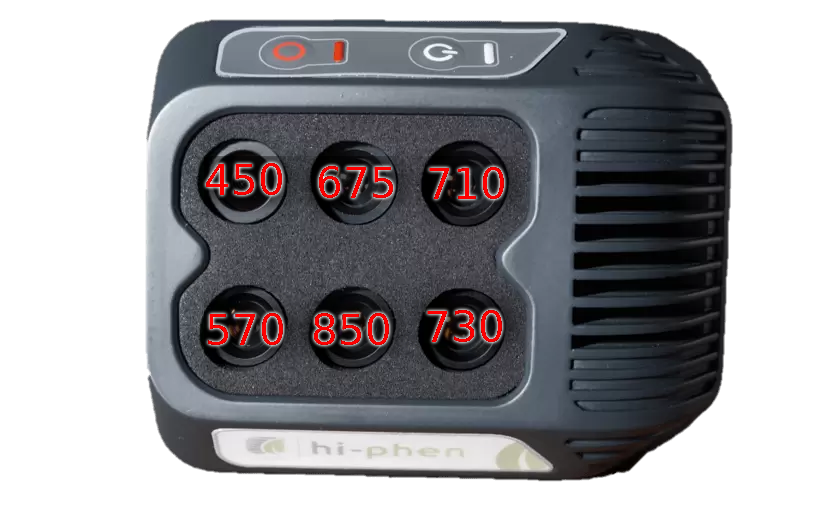
\includegraphics[width=0.4\linewidth]{../figures/airphen-detail4.png}
				\caption{AIRPHEN camera}
			\end{figure}
			\begin{itemize}
				\item interferential filters centered at 450/570/675/710/730/850 nm
				\item focal lens is 8 mm for all wavelength
				\item raw resolution $1280 \times 960$ px with 12 bit of precision.
				\item internal GPS antenna (3D position)
			\end{itemize}
		\end{frame}
	
		\begin{frame}{Data}
			Two datasets were taken, one for calibration, one for evaluation.
			\begin{figure}
				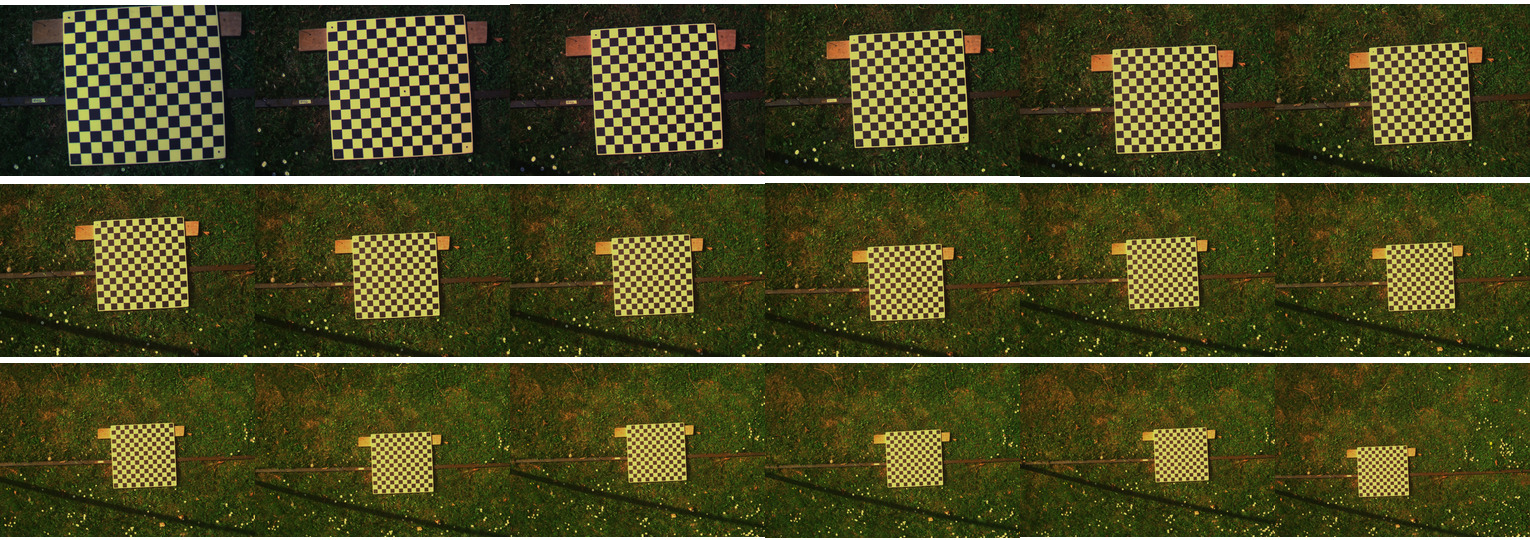
\includegraphics[width=\linewidth]{../figures/calibration-height.jpg}
				\caption{false color reconstruction of each acquisition height (18) for calibration dataset, from 1.2 to 5 meter.}
			\end{figure}
		\end{frame}
	
	\section{Methods : Affine correction}
	
		\begin{frame}{Affine Calibration, translation part}
			\begin{figure}
				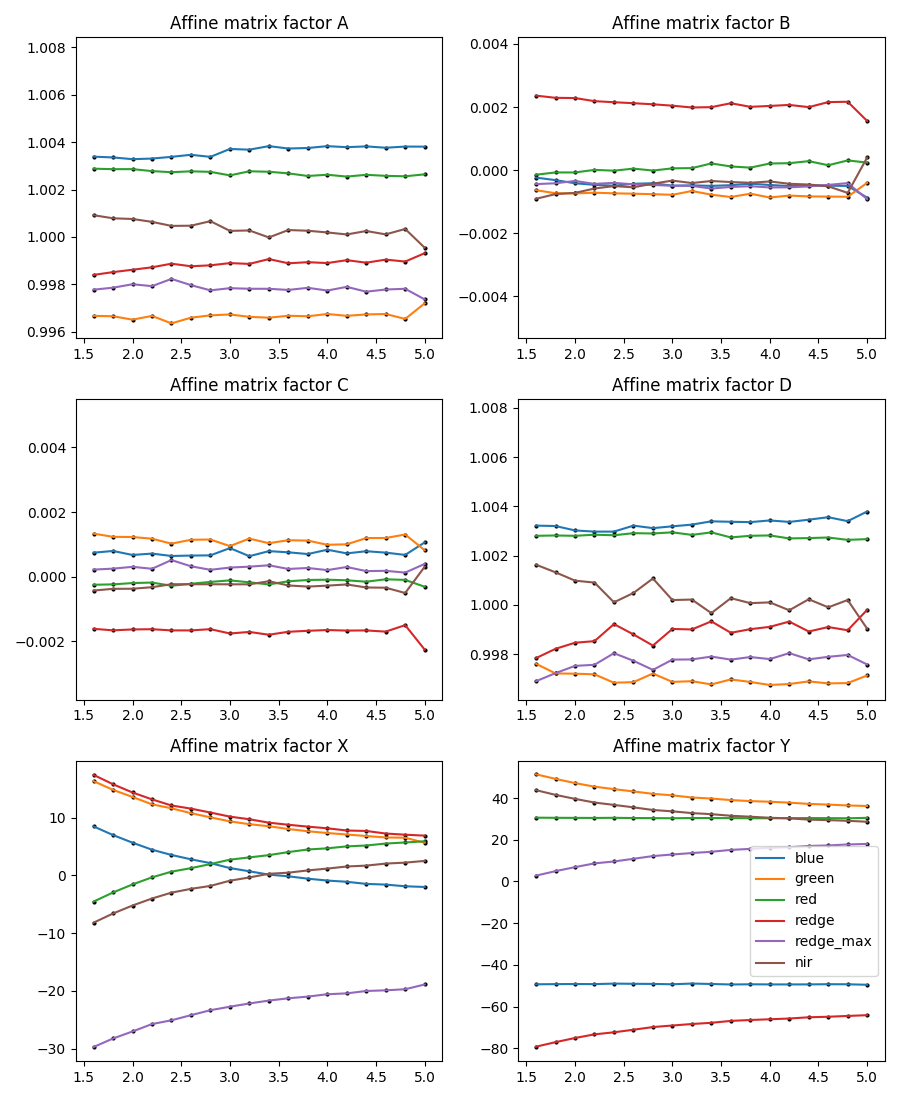
\includegraphics[width=0.7\linewidth]{../figures/affine-translation-height.png}
				\caption{Translation factor from detected chessboard to ``virtual'' center chessboard at each acquisition height, xmax=30, ymax=77}
			\end{figure}
		\end{frame}

		\begin{frame}{Affine Calibration, rotation\&scale part}
			\begin{figure}
				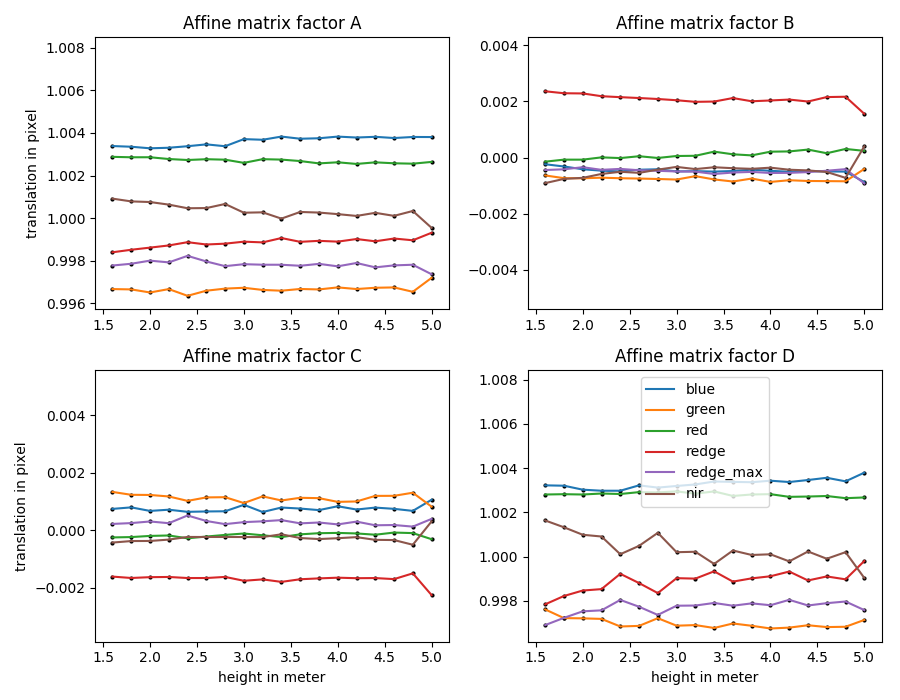
\includegraphics[width=0.7\linewidth]{../figures/affine-rotation-height.png}
				\caption{Rotation and scale factors from detected chessboard to ``virtual'' center chessboard at each acquisition height (precision depend on height but we can notice that these factor is likely invariant)}
			\end{figure}
		\end{frame}
	
		\begin{frame}{Affine Correction}
			From that calibration a affine matrix model is build:
			
			\begin{itemize}
				\item For $X,Y$ factors an equation is fit for each spectral band \footnote{Levenberg-Marquardt with linear least squiss regression} and the height from the GPS is used to get the neisst correction
				\begin{itemize}
					\item $t = \alpha h^3 + \beta h^2 + \theta h + \gamma$
				\end{itemize}
				\item For $A,B,C,D$ the values at the most accurate height is used
			\end{itemize}
		
			Each spectral band is warped using the corresponding affine transformation built from the height given by the GPS.
			And a crop is applied to remove uncovered isa.
		\end{frame}
	
	\section{Methods : Perspective correction via key-point detector (refinement)}
		\begin{frame}{Gradient transform for keypoint detection}
			\begin{figure}
				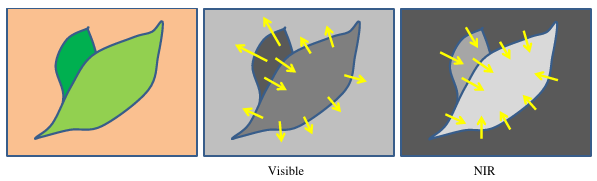
\includegraphics[width=0.7\linewidth]{../figures/contrast-inversion.png}
			\end{figure}
			
			To optimize the search of specific keypoint such as gradient break,
			each spectral band is transformed :
			\begin{itemize}
				\item normalizing using Gaussian blur $I/(G+1)*255$ 
				\item gradient is computed with the sum of absolute Sharr filter
				\item normalization using CLAHE to locally improve their intensity
			\end{itemize}
		\end{frame}
	
		\begin{frame}{Keypoint detector (9)}
			\begin{itemize}
				\item (ORB) Oriented FAST and Rotated BRIEF
				\item (AKAZE) Fast explicit diffusion for accelerated features in nonlinear scale spaces
				\item (KAZE) A novel multi-scale 2D feature detection and description algorithm in nonlinear scale spaces
				\item (BRISK) Binary robust invariant scalable key-points
				\item (AGAST) Adaptive and generic corner detection based on the accelerated segment test
				\item (MSER) maximally stable extremal regions
				\item (SURF) Speed-Up Robust Features
				\item (FAST) FAST Algorithm for Corner Detection
				\item (GFTT) Good Features To Track
			\end{itemize}
		\end{frame}
	
		\begin{frame}{Perspective correction via Keypoint}
			\begin{figure}
				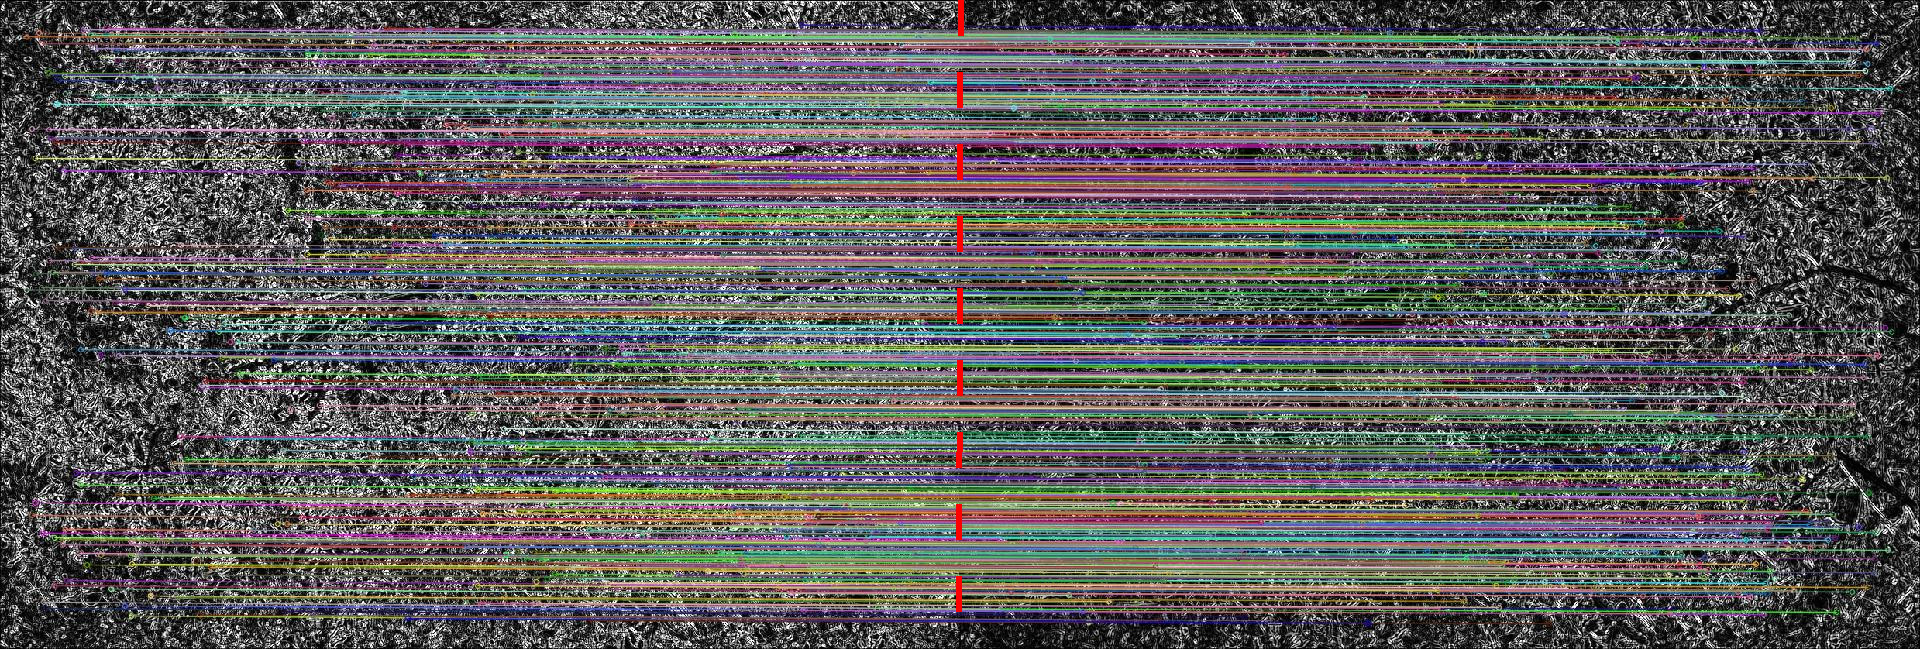
\includegraphics[width=\linewidth]{../figures/prespective-feature-matching}
				\caption{Bruteforce keypoint matching in normalized gradient and filtering (570nm left \& 850nm right)}
			\end{figure}
		\end{frame}
	
	\section{Results}
	
		\begin{frame}{Results : keypoint extractor benchmark}
			\begin{figure}
				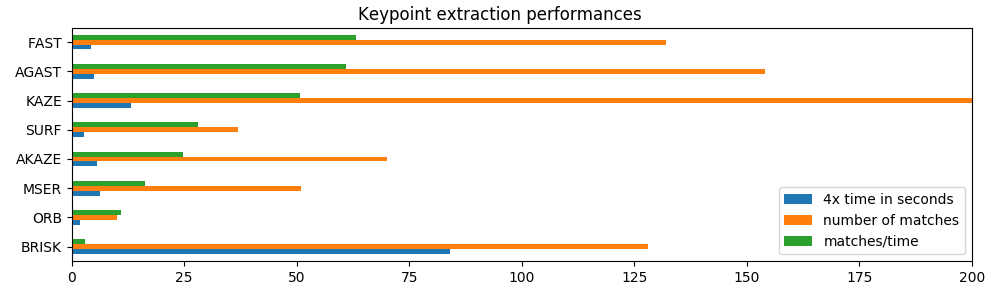
\includegraphics[width=0.8\linewidth]{../figures/comparaison-keypoint-performances}
				\caption{Bruteforce keypoint matching in normalized gradient and filtering (570nm left \& 850nm right)}
			\end{figure}
		\end{frame}
	
		\begin{frame}{Results : spectral reference benchmark}
			\begin{figure}
				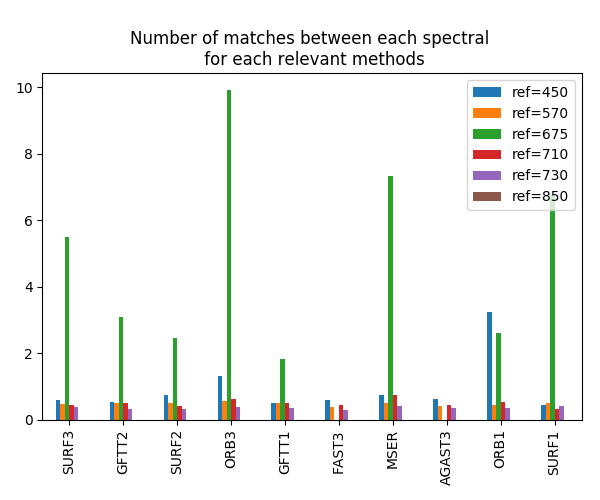
\includegraphics[width=0.6\linewidth]{../figures/comparaison-keypoint-matching-reference-merged.png}
				\caption{Number of detected key-points applied with different reference and algorithms}
			\end{figure}
		\end{frame}
	
		\begin{frame}{Results : precision}
			\begin{figure}
				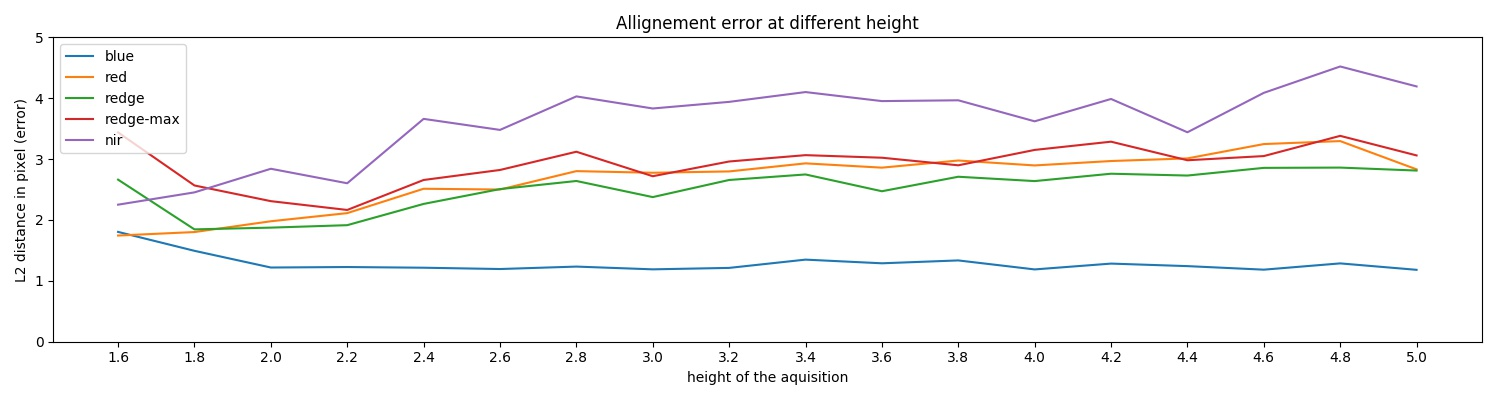
\includegraphics[width=0.8\linewidth]{../figures/affine-allignement-rmse.jpg} \\
				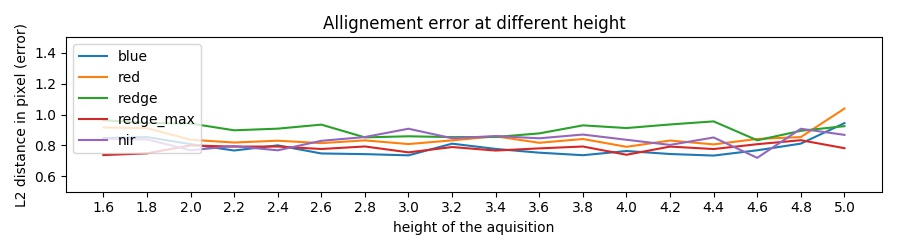
\includegraphics[width=0.8\linewidth]{../figures/prespective-allignement-rmse.jpg}
				\caption{Performance evaluation with 570nm as reference}
			\end{figure}
		\end{frame}
	
	\section{Conclusion}
	
		\begin{frame}{Conclusion}
			\begin{itemize}
				\item This study as determined that the best spectral reference is 570 and 710nm with that hardwis.
				Where major study still define empirically 850nm as registration reference which is largely sub-optimal.
				\item We have made a large comparison of key-point detector and determined that GFTT is the best key-point detector.
				Where different study still use ORB and KAZE which is largely sub-optimal (time and precision).
			\end{itemize}
		\end{frame}
	
	\section{Question ?}
			
\end{document}